\documentclass[12pt,a4paper]{article}
\usepackage[utf8]{inputenc}
\usepackage[french]{babel}
\usepackage[T1]{fontenc}
\usepackage{amsmath}
\usepackage{amsfonts}
\usepackage{amssymb}
\usepackage{graphicx}
\usepackage{url}
\begin{document}


\title{Mémoire de DEM \\ Utilisation de systèmes chaotiques pour la synthèse sonore.}
\author{Axel Chemla--Romeu-Santos}
\maketitle


La synthèse sonore, que ce soit dans le domaine analogique ou numérique, est contrôlée par le musicien grâce à un ensemble de paramètres. L'ensemble des paramètres d'un procédé de synthèse, afin que les répercussions qu'ils ont sur le son produit, définissent entièrement l'interaction que celui-ci crée avec l'utilisateur et le potentiel artistique qu'il confère. Le contrôle de ces paramètres est généralement effectué de manière manuelle ou séquencée, mais peut-être aussi effectué par d'autres générateurs, comme des oscillateurs basse-fréquence (LFO) ou des enveloppes temporelles. Ces générateurs permettent ainsi d'avoir un contrôle plus complexe sur le son généré, au prix de quelques paramètres additionnels. \\

Néanmoins, ces générateurs de paramètres ont souvent un comportement  relativement basique, et il pourrait être intéressant de développer des générateurs possédant des comportements plus complexes et peut-être plus à même d'exciter l'imagination de ses utilisateurs. Dans ce mémoire, nous proposons quelques pistes pour appliquer des objets mathématiques issus de la théorie du chaos. Ces objets peuvent se révéler intéressants car ils ont en commun un comportement dit \textit{chaotique}, c'est à dire hautement sensible à leurs conditions initiales et capable d'exhiber une infinité de comportements différents, au prix d'un nombre très restreint de paramètres. Certains de ces objets peuvent ainsi développer un comportent asymptotique, cyclique ou chaotique par une micro-variations de ses paramètres, permettant ainsi l'exploitation de combinaisons complexes à l'utilisateur.\\
Dans un premier temps, nous présenterons succinctement quelques notions principales de la théorie du chaos, ainsi que quelques objets chaotiques qui nous semblent intéressants dans une visée musicale. Ensuite, nous proposerons par la suite quelques exemples d'applications musicales.  

\section{Théorie du chaos}

\paragraph{Rapide historique.} La théorie du chaos, bien que formalisée dans les années 70 notamment par des scientifiques comme Lorenz, Thom et bien d'autres, s'inscrit en réalité dans une grande mouvance apparue dès la fin du XIX\textsuperscript{ème} siècle lors de l'étude des systèmes dits \textit{dynamiques}, c'est à dire dépendant du temps. Effectivement, l'observation toujours plus poussée de la nature dévoilait des comportements toujours plus complexes, amenant la recherche scientifique à relativiser un déterminisme strict et donc à adopter de nouveaux outils d'analyse. \\

Le premier cas rétrospectivement considéré comme ayant un comportement chaotique fut observé par Raymond Poincaré, tandis qu'il analysait les orbites respectives de la Lune, de la Terre et du Soleil (le \textit{problème à 3 corps}). Ces trajectoires, bien que non-périodiques, n'exhibaient pas non plus un comportement convergent (tendant vers un point fixe) ni divergent (l'écart entre les trajectoires n'augmentant pas avec le temps). Ce comportement inédit à l'époque fut l'un des premiers contacts scientifiques avec des objets dont le comportement était inconnu à l'époque : bien que déterministes au sens strict du terme, leur \textit{réalisation} était tellement sensible aux conditions initiales que leur prédiction exacte était impossible. \\
 Parallèlement, l'analyse du comportement des gaz par des scientifiques comme les fameux Maxwell, Kelvin et Boltzmann forçait les scientifiques à délaisser un déterminisme rigoureux pour une description probabiliste de l'état des particules au cours du temps, donnant ainsi naissance à la \textit{physique statistique}. Contrairement à la mécanique newtonienne classique où l'étude du mouvement de l'objet était caractérisable (du moins en théorie) par ses conditions initiales et la structure du système, le parcours d'une particule de gaz se révélait totalement imprévisible, obéissant à un mouvement dit brownien (du bruit pur). Néanmoins, la caractérisation de l'\textit{état} d'un gaz pouvait être donné en étudiant la \textit{probabilité} de la position d'une particule, qui ne varie pas dans une situation d'équilibre. Là aussi, on se retrouvait à devoir caractériser des corps dont la réalisation est \textit{de-facto} imprévisible, mais dont la caractérisation peut-être donné un analysant leur état. \\
 
Dans les deux cas, les scientifiques eurent donc un premier contact avec des systèmes dynamiques dont la description mathématique classique ne suffisaient plus. Dans la mesure où ces comportements apparaissaient de même dans l'étude d'équations différentielles non-linéaires, l'analyse des systèmes dynamiques devint donc une champ d'études très actif avec notamment des scientifiques comme Hopf et Lyapunov, qui donnèrent le jour à des notions et outils que les scientifiques utilisent encore aujourd'hui.\\

Néanmoins, la formalisation d'une "théorie du chaos" vint bien plus tard grâce à l'apparition des ordinateurs, permettant le calcul plus rapide de certaines de ces trajectoires. La naissance "formelle" de la théorie du chaos et datée des découvertes de Lorenz dans le domaine de la météorologie dans les années 60, à qui l'on doit la fameuse métaphore du papiillon déclenchant un ouragan. L'étude qu'il fit de l'objet qu'il a découvert, \textit{l'attracteur de Lorenz}, ouvrit la porte à une méthode d'analyse de ces modèles, souvent définis par récurrence, basés sur les recherches de Poincaré. Parallèlement, les études de Mandelbrot sur les fractales (qui sont des objets chaotiques) participèrent à rendre ce champ d'étude populaire, aidé par le fait que sa généralité lui permettait d'être appliqué à un grand nombre de champs d'étude (météorologie, électronique, modélisation de comportements, finance...). Finalement, la notion de \textit{chaos} fut crée en 1975 par Yi \& Yorke, donnant ainsi un nom à cette théorie. Encore étudiée aujourd'hui, cette discipline a également fait de nombreux enfants (telle la \textit{théorie des catastrophes} de René Thom) et fait partie des théories les plus importantes du XX\textsuperscript{ème} siècle.


\paragraph{Théorie des comportements chaotiques et méthode d'analyse.}
Un système \textit{chaotique} est donc un système dynamique, qui dépend donc du temps. Il existe deux catégories de temporalité : une temporalité \textit{discrète}, où les termes de la suite se calculent de manière successive, ou bien une temporalité \textit{continue}, où le temps n'est pas divisé en étape mais est considéré comme un axe lisse. Il existe plusieurs critères pour définir un objet comme chaotique ;  néanmoins, les plus admis sont les critères suivants :\\


\begin{itemize}
\item \textit{sensibilité} aux conditions initiales : une petite différence dans la condition initiale peut modifier à grande échelle le comportement du système
\item \textit{mélange topologique} : les positions probables d'un système donné sont les même au cours du temps
\item \textit{récurrence} : à chaque étape, l'étape suivante est calculée en fonction des précédentes \\
\end{itemize}

À titre d'exemple, nous allons prendre le plus simple (et donc un des plus fascinant) example de système chaotique : la \textit{suite logistique}. Cette suite, dont l'expression est extrêmement simple, est calculée récursivement et dépend d'un seul paramètre $\mu$ :

\[
x[n+1] = \mu \cdot x[n] \cdot ( 1 - x[n])
\]
chaque nouveau terme de la suite est donc calculée en fonction du terme précédent et de la valeur du paramètre $\mu$, que nous sommes libre de choisir librement. En observant la suite obtenue en faisant varier le seul paramètre $\mu$, on peut observer que cette suite peut prendre des morphologies radicalement différentes (voir fig. \ref{logistic}).\\

\begin{figure}
\begin{center}
\label{logistic}
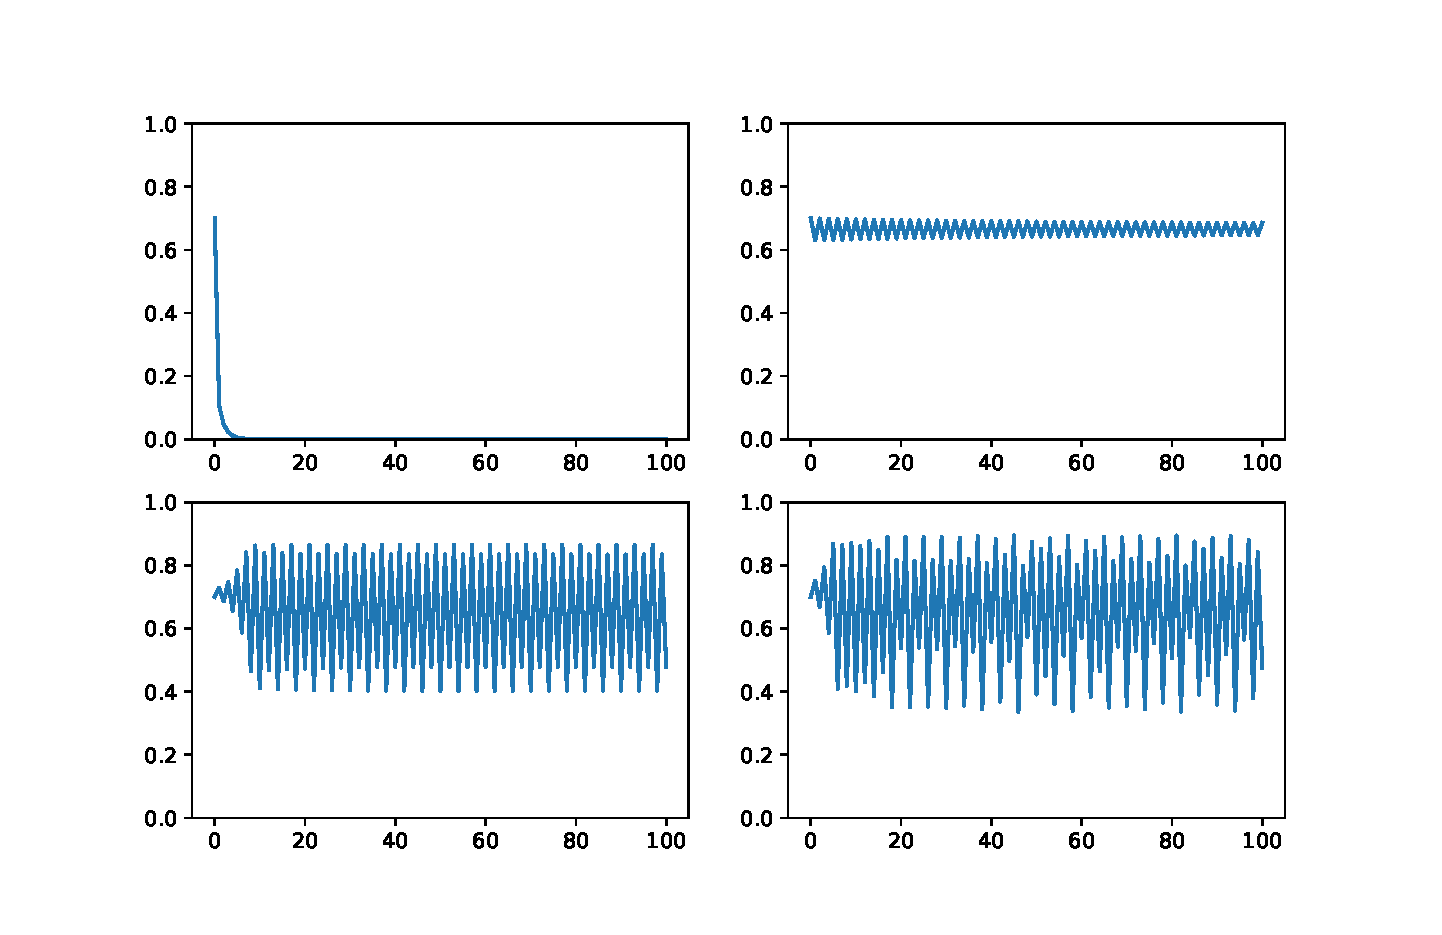
\includegraphics[scale=0.5]{medias/logistic_figs.eps}
\caption{Tracé de suite logistique pour $\mu = 0.5, 3, 3.47, 3.58$}
\end{center}
\end{figure}

Cette suite, dont le comportement a été depuis largement étudié grâce à la simplicité de sa paramétrisation, se comporte de la manière suivante : 
\begin{itemize}
\item $0 \leq \mu \leq 1$ : la suite converge vers 0.
\item $1 \leq \mu \leq 2$ : la suite se stabilise autour de $(\mu -1)/ \mu$.
\item $2 \leq \mu \leq 3$ : la suite converge toujours vers $(\mu -1)/ \mu$, mais oscille pendant quelques étapes autour de cette valeur ; plus $\mu \rightarrow 3$, plus la vitesse de convergence est lente
\item  $2 \leq \mu \leq 3.57$ selon la valeur de $\mu$ la suite oscille entre deux valeurs, puis quatre, puis huit, jusqu'à un nombre presque infini de cycles
\item $\mu > 3.57$ la suite est \textit{presque toujours} chaotique.
\end{itemize}
On peut donc constater que, en jouant sur le seul paramètre $\mu$, cette suite peut développer des comportement radicalement différents. 

\begin{figure}
\begin{center}
\label{phases}
\includegraphics[scale=0.4]{medias/phase_logistique.png}
\includegraphics[scale=0.05]{medias/lorenz_attractor.jpg}
\caption{Espace de phases pour la suite logistique en fonction de plusieurs paramètres  $\mu$ (gauche) et pour un attracteur de Lorenz (droite)}
\end{center}
\end{figure}

\paragraph{Méthodes d'analyse.} Afin de caractériser ces objets chaotiques, plusieurs méthodes d'analyse furent développées. La plus ancienne et la plus connue est la notion de \textit{stabilité de Lyapunov}, qui quantifie la "chaoticité" d'un système en mesurant la différence moyenne des réalisations obtenues avec deux conditions initiales très proches. Néanmoins, il est plus souhaitable dans un cadre musical d'avoir une représentation plus intuitive.
La façon la plus directe d'obtenir une compréhension sur la structure d'un système chaotique est d'observer la valeur dans l'\textit{espace des phases}, c'est à dire s'affranchir du temps pour observer les valeurs que prennent les objets chaotiques afin d'en dégager la structure. L'espace des phases, défini sur ligne pour la suite logistique car unidimensionnelle, est visible figure \ref{phases} : sont notés par un trait vertical les différentes valeurs prises par la suite pour plusieurs $\mu$. Est aussi affiché le diagramme de phase d'un attracteur de Lorenz, un autre système chaotique mais qui est lui en trois dimensions \footnote{\url{https://upload.wikimedia.org/wikipedia/commons/e/ef/Lorenz_attractor_boxed.svg}} On peut voir que ces graphiques nous livrent de précieuses informations sur la structure des objets et les valeurs qu'il prennent au cours du temps, même si ceux-ci ont un comportement complexe. \\

Une autre méthode pour comprendre le comportement d'un objet chaotique est de tracer son \textit{diagramme de bifurcation}. De manière similaire, nous nous affranchissions du temps mais nous traçons les différentes valeurs possibles de la suite en fonction de leurs paramètres. On peut voir figure \ref{bifurcation} le digramme de bifurcation de la suite logistique ; on peut voir que, pour $\mu > 2$, il y'a deux valeurs possibles, et que le nombre de valeurs possibles augmente sévèrement jusqu'à $3.57$, ou toutes les valeurs sont possibles. Ces diagrammes peuvent donc être utiles pour obtenir une compréhension directe du comportement chaotique d'un système dynamique. 



\begin{figure}
\begin{center}
\label{bifurcation}
\includegraphics[scale=0.15]{medias/logistic_bifurcation.png}
\caption{Diagramme de bifurcation de la suite logistique}
\end{center}
\end{figure}



\section{Exemples d'applications musicales}
Nous allons maintenant dégager quelques pistes et présenter quelques exemples du l'usage actuel des système chaotiques pour la synthèse sonore. Ces systèmes se révèlent intéressants par la diversité des comportements qu'il peuvent adopter pour un nombre limité de paramètres ; nous allons donc nous employer à utiliser cette richesse dans la contrôle de procédés de synthèse. Les exemples sonores sont disponibles à l'adresse suivante : \url{https://github.com/domkirke/chaotic-control}

\subsection{Utilisation de la suite logistique}
Pour montrer l'intérêt de l'usage de générateurs de contrôle chaotiques, nous allons dans un premier temps analyser les potentialités ouvertes par cette simple suite logistique présentée ci-dessus. Afin de pouvoir extraire le meilleure usage de cette suite, il nous en faut dégager les principales caractéristiques :
\begin{itemize}
\item elle est à temps discret, c'est à dire qu'elle est organisée en états successifs $n$, $n+1$, ...
\item elle peut présenter un comportement asymptotique, cyclique ou chaotique.
\end{itemize}
Nous allons donc utiliser ces propriétés pour proposer plusieurs applications de son usage.

\paragraph{Génération de séquence.} Dans la mesure où cette suite est à temps discret, une de ses applications immédiates est la synthèse de séquence, à la manière d'un arpégiateur. Néanmoins, dans la mesure ou cette séquence donne des valeurs dans un espace continu entre 0 et 1, cela inclut de découper cet intervalle en échelles afin de pouvoir en extraire une séquence. Nous donnons plusieurs exemples d'application : 
\begin{itemize}
\item Dans le premier exemple, nous discrétisons l'espace entre 0 et 1 en sept valeurs, de manière à sortir des valeurs sur une échelle heptatonique.
\item Dans le second exemple, nous discrétisons l'intervalle [0, 1] et utilisons les comportements cycliques de la suite logistique de manière à générer des rythmes. 
\end{itemize}
Dans ces applications nous calculons les valeurs successives de la suite à intervalle réguliers. Néanmoins, il est possible d'agencer de manière plus complexe cette temporalité.

\paragraph{Génération de paramètres.} Il est aussi possible d'utiliser l'intervalle [0,1] sans le discrétiser afin de contrôler de manière continue les paramètres de la synthèse sonore. Néanmoins, comme la suite logistique est basée sur un temps discret, celà peut inclure le \textit{lissage} de la suite grâce à une interpolation linéaire (relier les points successifs par des droites continues) afin pouvoir contrôler un paramètre de manière continue. De même nous présentons plusieurs exemples d'application :
\begin{itemize}
\item Nous utilisons le régime $ 2 < \mu < 3$, dont la caractéristique est de converger à valeurs différentes, pour contrôler la fréquence de chaque composante d'un synthétiseur polyphonique, comme une sorte d'unison dynamique. 
\item Nous utilisons les valeurs sorties par la suite logistique pour contrôler des enveloppes temporelles, ou nous déclenchons la sortie de chaque nouveau terme de la suite dès que l'enveloppe précédente est terminée. Cela permet d'utiliser pleinement la sortie continue de la suite, tout en l'utilisant elle-même pour gérer sa temporalité.
\end{itemize}

Nous pouvons voir que en dépit de sa simplicité cette suite permet de nombreuses applications intéressantes et qu'elle permet de raisonner plus en terme de \textit{comportement} et de laisser libre cours à leur complexité. 

\subsection{Conjecture de Collatz.}
Ici nous présenterons brièvement la conjecture de \textit{Collatz} ou de \textit{Syracuse}, dont les propriétés nous ont intéressés d'un point de vue musical. Partant d'une condition initiale $u_0 = N$ ou $N$ est un nombre entier, la suite suivante est calculée : 

\[
u_{n+1} = \begin{cases} \frac{u_n}{2} \text{ si } u_n \text{ est pair} \\
3 u_n + 1  \text{ si } u_n \text{ est impair} \end{cases}
\]

Dans tous les cas, cette suite termine par converger vers un cycle (1, 2, 4) ; néanmoins, c'est le temps qu'elle mets à y arriver qui nous intéresse ici. Ce temps de convergence, appelé \textit{temps de vol} que l'on définit par le temps que la suite met à atteindre la valeur 1, est extrêmement variable en fonction de la valeur initiale $N$.\\

D'un point de vue musical, ce qui nous intéresse ici est la forme globale de la phase transitoire de cette suite, dont nous nous servons comme enveloppe temporelle (nous arrêtons l'enveloppe dès que la première valeur 1) est atteinte. Nous montrons fig. les formes de cette enveloppe pour des valeurs très proches de $N$, et de la même manière que la suite logistique cette diversité peut-être obtenue en agissant uniquement sur le paramètre $N$. Nous donnons une application sonore de cette enveloppe dans le contexte de la synthèse FM, où nous l'affectons à l'amplitude de la modulation. Dans la mesure ou ce générateur est une suite, nous utilisons  aussi une interpolation linéaire afin de pouvoir contrôler le paramètre de manière continue.


\subsection{Attracteur de Lorenz}
Enfin nous présentons une application d'un système chaotique plus complexe, la conjecture de Lorenz, dont l'espace des phases est montré \ref{phases}. Contrairement aux systèmes dynamiques utilisés précédemment, l'attracteur de Lorenz est à temps continu et tri-dimensionnel, ce que signifie que le système donne trois valeurs à la fois. Cela permet de lier par le même système plusieurs paramètres et ainsi de les faire interagir de manière complexe. De plus, le fait que l'attracteur de Lorenz permet un contrôle continu de ses paramètres, contrairement au système précédent ou le déclenchement de chaque nouvel élément de la suite devait être ordonnancé.\\

En analysant l'espace de phase de l'attracteur de Lorenz, nous pouvons voir qu'il "tourne" autour de deux points, nommés \textit{attracteurs étranges}, d'une manière constamment différente par rapport à tours précédents. Nous pouvons donc imaginer les attracteurs de Lorenz comme une manière contenu de faire tourner un ensemble de paramètres autour d'une même configuration, dont ils s'approcheront toujours de manière différente sans jamais l'atteindre. De même, comme cet attracteur doit se connecter à deux ou trois paramètres, il faut choisir judicieusement ces deux paramètres afin que cette interaction puisse être perceptivement audible. Nous proposons donc plusieurs pistes pour l'usage de l'attracteur de Lorenz dans la synthèse sonore : \\

\begin{itemize}
\item \textit{application à la synthèse granulaire} : on choisit d'utiliser un attracteur de Lorenz afin de régler, avec le même générateur, la taille de fenêtre et la position dans le fichier de la recomposition granulaire d'un son.
\item \textit{oscillateurs inter-pénétrés} : il est aussi possible d'utiliser les plusieurs valeurs sorties par l'attracteur de Lorenz afin de lier ensemble plus synthétiseurs : nous essayons cette effet là en interconnectant deux moteurs de synthèse FM, ou l'amplitude et la fréquence de la modulation de fréquence sont connectées au même attracteur mais en miroir. \\
\end{itemize}

Les attracteurs de Lorenz sont basés sur trois paramètres, dont seul un agit principalement sur sa morphologie. Grâce à cet attracteur, il est donc possible de lier au minimum trois paramètres par une interaction complexe en agissant sur un seul paramètre. Similairement aux attracteurs de Lorentz, d'autres attracteurs tels les attracteurs de Duffing, ou de Clifford, ayant chacune des morphologies diverses avec un nombre réduit de paramètres.


\subsection{Autres applications musicales}
Au-delà de l'application de ces phénomènes chaotiques au contrôle pour la synthèse sonore dont nous parlons ci-dessus, la théorie du chaos est déjà présente dans certaines applications musicales.

\paragraph{Équations différentielles non-linéaires.} La théorie du chaos apparaît naturellement lors de l'analyse des équations différentielles non-linéaires, qui apparaissent naturellement lors de l'analyse mécanique de certains instruments de musique. Dans la mesure où n'importe quel corps vibrant idéalisé peut-être modélisé avec une équation différentielle du second degré, l'introduction de termes non-linéaire correspondant par exemple à des perturbations, des phénomènes de frottement  ou encore des oscillations forcées placent en général l'équation modélisée en régime chaotique. Ce comportement est par exemple connu dans le cas du violon (dont l'oscillation est forcée par l'archet), où l'on peut comparer le régime bruiteux lors d'une pression forte de l'archet avec le cycle aléatoire de la suite logistique présentée ci-dessus. 

\paragraph{Caractérisation de circuits analogiques.}  Des outils issus de la théorie ergodique et de la théorie du chaos sont aussi très utilisés dans la caractérisation de système analogiques, notamment pour la production sonore. Une des premières découvertes dans ce sens fut l'étude de \textit{l'oscillateur de Van der Pol}, qui servit de base à l'étude des phénomènes complexes amenés par les systèmes électroniques amplifiés. Ainsi, les circuits hautement non-linéaires (analysés grâce au \textit{séries de Volterra}) ont une certaine tendance à développer des comportements chaotiques, ce qui est certainement l'origine du caractère \textit{analogique} tant apprécié dans les années 60.


\section{Conclusion}
Nous avons donc brièvement expliqué les propriétés fondamentales de la théorie du chaos, ainsi présenté quelques propriétés de base de ces systèmes. Nous avons aussi pris les cas particuliers de la suite logistique, la conjecture de Collatz et l'attracteur de Lorenz, et présenté quelques usages possibles pour contrôler des paramètres de synthèse sonore. Ces systèmes dynamiques très simples pouvant développer un grand nombre de comportements complexes, nous avons donc montrer que ces générateurs chaotiques peuvent être fort intéressants pour ce genre de contrôle et peuvent donc complètement trouver leur place à côté des LFOs ou des enveloppes dans les outils de base pour le contrôle de la synthèse.


 
 
\end{document}